\mychapter{1}{\textgamma+jet event classification in LHC collisions}
\label{chap:premierchapitre}

\section{CMS experiment at LHC}

The Compact Muon Solenoid (CMS) fig (\ref{cms}) is a particle physics detector built at one of the collision points of the Large Hadron Collider
(LHC) at CERN in Switzerland and France. The goal of the CMS experiment is to investigate the physics of the Standard Model and beyond.
CMS is designed as a general-purpose detector, capable of studying many aspects of proton collisions at 0.9-13 TeV, the
center-of-mass energy range of the LHC particle accelerator.\\
CMS is made of multiple particle detectors designed to measure the energy and momentum of products of the collisions.
The innermost layer called the "Tracker" reconstruct the paths of charged particles comming from the collision or from the
decay of short-lived particles.
%high-energy muons, electrons and hadrons as well as see
%tracks coming from the decay of very short-lived particles.\\
Next the "Electromagnetic Calorimeter" is designed to measure with high accuracy the energies of electrons and
photons.\\
The Hadronic Calorimeter measures the energy of hadrons.%and provides indirect measurement of the presence of
%non-interacting, uncharged particles such as neutrinos.\\
Theses layers all fit inside a large solenoid magnet generating in its inner part a magnetic field of 3.8 Tesla, this allows the charge/mass ratio of particles to be
determined from the curved track that they follow in the magnetic field.
Finally, the magetic field flux return yoke, outside the solenoid, is instrumented with muon detectors \cite{CMS2008}.

\begin{figure}[h!]
  \centering
  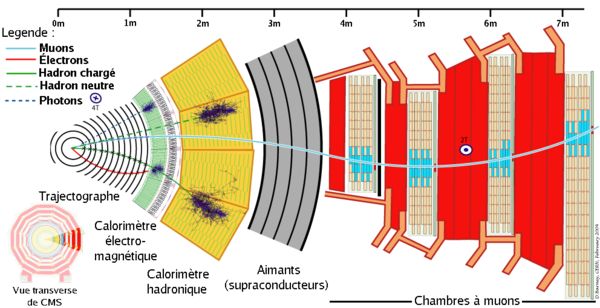
\includegraphics[width=0.8\textwidth]{cms}\\[1cm]
  \caption{Diagram of a slice of the CMS detector, from left to right : tracker, electromagnetic calorimeter, hadronic
  calorimeter, superconductive solenoid and muon chamber. Lines represent track of particles.}
  \label{cms}
\end{figure}


\section{Pile-up events}

At the LHC protons are bunched together, into up to 2808 bunches composed of around $10^{11}$ protons each.
When two bunches interact there is a non-negligeable probability that multiple events arise from this collision, these
are called pile-up events and have to be taken into account for particle reconstruction.

\section{CMS coordinate system}

The absolute CMS coordinate system is defined with respect to the LHC ring. The X axis points towards the center
of the ring, the Y axis points up and the Z axis is defined as per a right handed coordinate system. \\
The absolute azimuth \textphi runs from the X axis (at 0 degree) towards the Y axis and \texteta is the polar angle.\\
Initial energy of the particles is along the beam axis. Due to the energy conservation, the total energy in the plane
transverse to the beam axis has to be zero. For this reason, in the following we will always consider the transverse
momentum $\vec{p}_{T}$ (with $p_{T} = |\vec{p}_{T}|$).


\section{Hadronic jets in proton-proton collisions}

Jets are the experimental signatures of high-energy quarks and gluons produced in high-energy processes.\\
During proton-proton collisions high-energy quarks and gluons may be produced they will radiate high-energy gluons or
decay into high-energy quark-antiquark pairs (for gluons). This process is called a parton shower, a lot of quarks and
gluons are produced but these particles having a colour charge.\\
Thereby they cannot exist freely due to coulour-confinement and come together to form colour-neutral hadrons by a process called
hadronisation that leads to a collimated spray of hadrons called a hadronic jet.
The detailed understanding of both the jet transverse momentum scale and resolution is of crucial importance for many physics analyses.


%%% Local Variables: 
%%% mode: latex
%%% TeX-master: "isae-report-template"
%%% End: 
